
La espectroscopía es una técnica de análisis utilizada para determinar los componentes de una mezcla. A grandes rasgos se basa en el diferente comportamiento de los compuestos al absorber energía y volver a su estado natural al liberar la energía absorbida.
Dependiendo de la fuente energética para excitar los átomos de la materia podemos distinguir entre 4 clases de espectroscopía:

\begin{itemize}
 \item Espectroscopía de masas
 \item Espectroscopía de luz Ultravioleta-visible
 \item Espectroscopía de luz Infrarroja
 \item Espectroscopía de Resonancia Magnética Nuclear
\end{itemize}


En este capítulo nos centraremos en la espectroscopía de Resonancia Magnética  Nuclear (RMN). Esta técnica toma provecho de las propiedades del spin de los protones (de ahí su nombre), es la técnica más utilizada para la detección de moléculas orgánicas, y a pesar de que la espectroscopía se puede basar en diferentes átomos, la más utilizada es la espectroscopía de H, dado que su núcleo es un solo protón y este elemento se encuentra en gran proporción en componentes orgánicos y  presentes en el cuerpo.

A pesar de la gran popularidad actual de las técnicas de imagen por resonancia magnética (iRMN),  el uso de la resonancia magnética vino de la mano de la espectroscopía. La técnica de espectroscopía por RMN, a pesar de necesitar muestras mayores que las otras técnicas de espectroscopía, cuenta con la importante ventaja de ser  una técnica no destructiva, siendo posible que se desarrollase posteriormente la espectroscopía por RMN in vivo.

La espectroscopía RMN se basa en los mismos principios físicos implicados en la obtención de iRMN. En condiciones naturales los protones H presentan un spin que les concede un campo magnético propio, en presencia de un campo magnético externo, estos se pueden presentar de dos modos:
\begin{itemize}
 \item En su estado de menor energía. Alineado con el campo magnético externo (spin \nicefrac[]{1}{2}).
 \item En su estado de mayor energía. Opuesto al campo magnético externo (spin -\nicefrac[]{1}{2}).
\end{itemize}



La diferencia de energía entre estos dos estados es dependiente de la fuerza del campo magnético externo (B0) y es siempre muy pequeña. Los dos estados de spin son igualmente energéticos cuando el campo magnético externo es cero, no obstante la diferencia energética se incrementa a mayor fuerza del campo magnético externo.

\begin{figure}[htb]
 \begin{figg}
   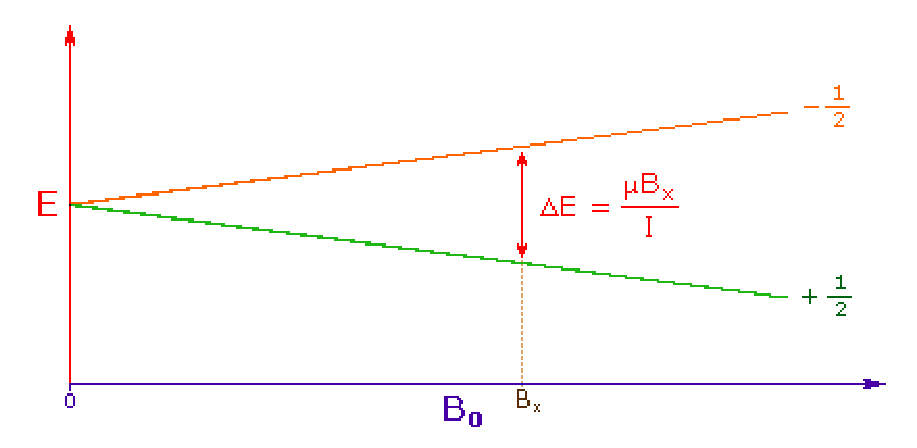
\includegraphics[width=0.7\textwidth]{espectro_deltaE}
   \caption{En el gráfico se muestra como aumentan la diferencia energética entre los dos estados de spin posible con el aumento del campo magnético \Bzero.}
 \label{fig:espectro_deltaE}
 \end{figg}
\end{figure}
 


Es por este fenómeno por el cual las técnicas de resonancia magnética requieren de potentes imanes con los que generar un fuerte campo magnético. La unidad para medir la fuerza del campo magnético del S.I. es el Tesla (T). 

En las técnicas actuales de espectroscopía se utiliza campos magnéticos de entre 1 y 20 T, pero a pesar de estos potentes campos magnéticos la diferencia entre los estados de spin es muy pequeña  (<0.1 cal/mol). 
La irradiación de una muestra con un pulso de radiofrecuencia (RF) que corresponda exactamente con la diferencia energética entre spines provocará el paso de la forma menos energética, \nicefrac[]{1}{2}, a la más energética, -\nicefrac[]{1}{2}. La diferencia entre los dos estados de spin es proporcional al momento magnético ($\mu$), siendo para H $\mu$ = 2.7927 magnetones nucleares.

Todos protones (H) tienen el  mismo momento magnético por tanto esperaríamos que todos nos dieran la misma señal. Pero de hecho, distintos protones se pueden comportar de forma distinta bajo las mismas condiciones del pulso de RF y magnetismo, cosa que nos permite discriminar entre ellos y da sentido a esta técnica analítica.

Cuando ponemos una muestra en el resonador, esta no está compuesta puramente de protones (H). Los ``protones'' que medimos se encuentran rodeados por electrones, que forman uniones de tipo covalente e iónicas, formando parte de moléculas. Los electrones son partículas cargadas negativamente, y por ello se mueven en respuesta al campo magnético externo aplicado (\Bzero) y generan un campo magnético secundario opuesto. Este campo magnético secundario opuesto amortigua el efecto del campo magnético externo sobre el núcleo. Es por ello que debemos tener en cuenta que el campo magnético efectivo (el que el núcleo ``siente'') será menor que le \Bzero, y que la pérdida de magnitud se debe al corrimiento químico ($\sigma$), el cual trataremos más adelante. 

\begin{equation}
 B = B_0 (1-\sigma)
\end{equation}

La densidad electrónica alrededor de cada átomo de una molécula varía con el tipo de núcleo y los enlaces que forma con otros átomos. El campo magnético opuesto de cada núcleo será diferente.



\begin{figure}[htb]
 \begin{figg}
   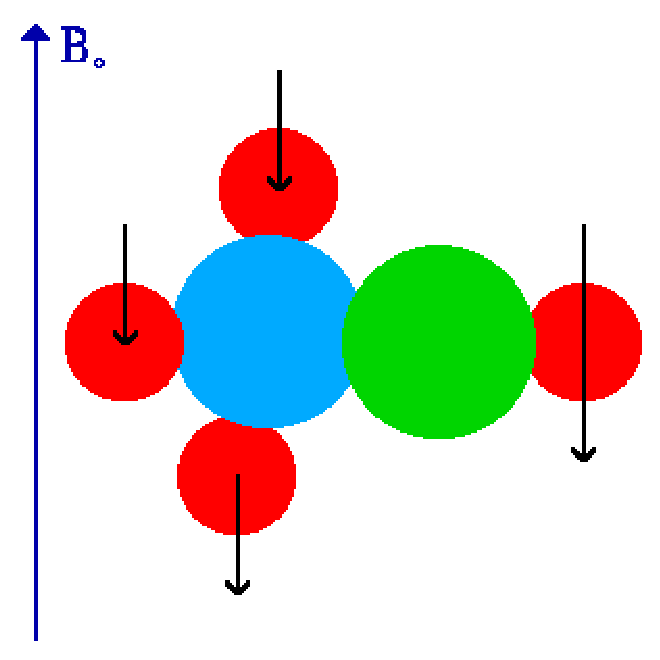
\includegraphics[width=0.7\textwidth]{espectro_metanol}
   \caption{En la imagen podemos observar una molécula de metanol en un campo magnético, \Bzero. En ella se aprecia como el H (en rojo) unido al átomo de oxigeno (O) (en verde) presenta un campo magnético opuesto mayor al de los H unidos al átomo de Carbono (C) (en azul).}
 \label{fig:espectro_metanol}
 \end{figg}
\end{figure}




La diferencia entre las frecuencias de resonancia de los protones depende del B0 (a mayor B0, mayor diferencia), esto hace que las diferencias de frecuencia no se puedan comparar con espectrofotómetros de diferentes teslajes (o incluso entre equipos distintos si consideramos que los imanes no serán exactamente iguales). 
Con la intención de resolver este problema se utiliza el corrimiento químico $\omega$. El corrimiento químico de un núcleo es la diferencia entre la frecuencia de resonancia de un núcleo y su estándar, relativo a un estándar:
\begin{equation}
 \omega = (\nu - \nu_{ref}) / \nu_{ref}
\end{equation}

Al igual que en imagen por RMN, la señal requiere la transformada de Fourier para distinguir entre los componentes de la mezcla (y sus respectivas señales). Dado que las diferencias de frecuencias son mínimas, el numerador se expresa en Hz, siendo el denominador expresado en MHz. Esto lleva a un ratio sin unidades $1/1x10^6$ (uno entre 1 millón), por lo que se expresa en unidades de ``partes por millón'' (ppm).

En espectroscopía de RMN usualmente se toma el compuesto tetrametilsilano, $Si(CH_3)_4$, (TMS), como valor de referencia; ya que es un compuesto químicamente inerte, puede ser fácilmente extraído de la mezcla y presenta una sola señal de RMN aguda (todos sus H presentan las mismas uniones) que  no interfiere con la resonancia de otros componentes orgánicos. Todos los protones (H) del TMS tienen el mismo patrón de uniones, por tanto darán todos la misma señal. Esta señal nos marcara el 0 en la escala de unidades de ppm para comparar con otros compuestos. 



\begin{figure}[htb]
 \begin{figg}
   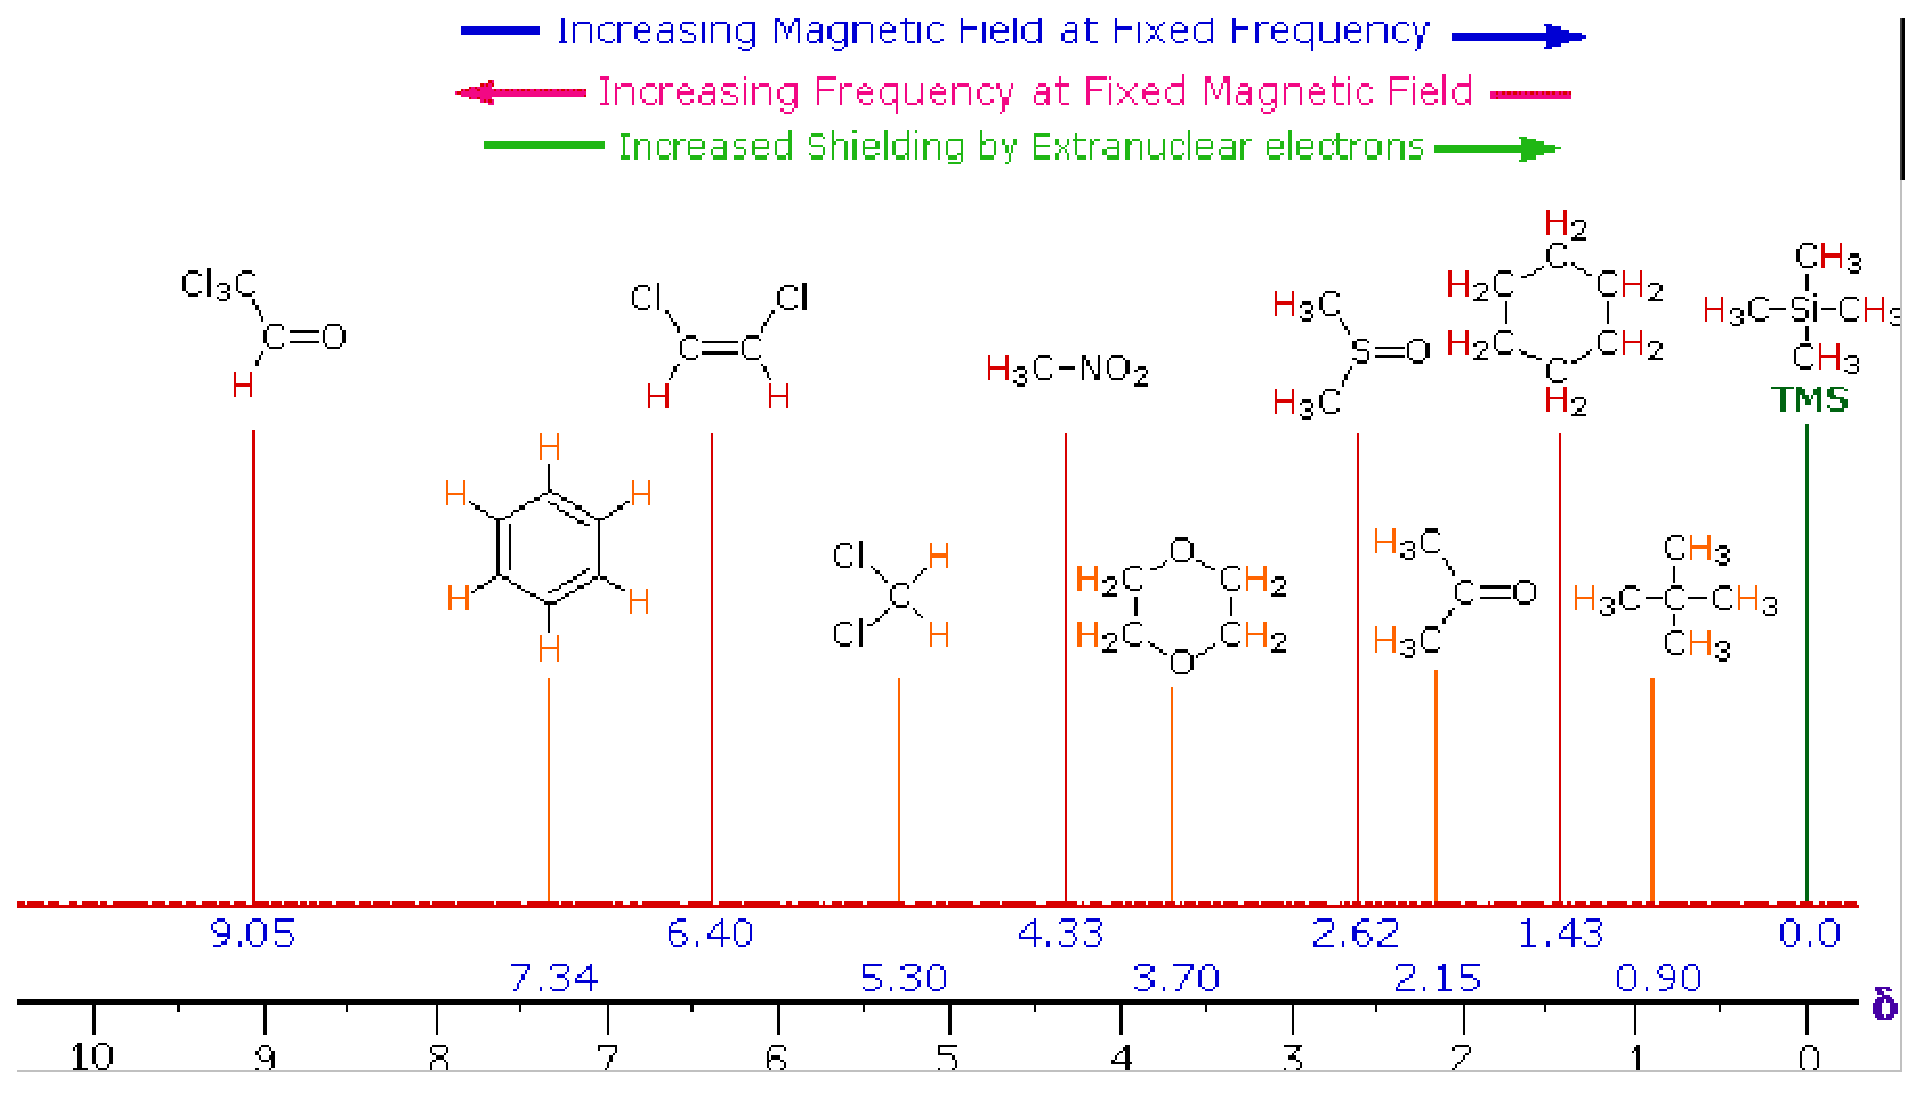
\includegraphics[width=\textwidth]{espectro_espectro}
   \caption{Falta pie de figura.}
 \label{fig:espectro_espectro}
 \end{figg}
\end{figure}


Como se mencionó anteriormente aquellos compuestos en que todos su H son estructuralmente equivalentes (mismo tipo de uniones con el mismo tipo de átomos) presentan una sola señal aguda de RMN. Por otro lado cuando esta condición no se cumpla, recibiremos una señal distinta por cada radical en el que esté involucrado un átomo de H. Dado que la técnica es incapaz de distinguir H equivalentes, la magnitud de la señal de RMN (representada en el eje de la y) es proporcional a la concentración molar de dichos protones en la muestra. Es decir a mayor intensidad de la señal, mayor será el número de H con la misma sigma y por tanto unidos al mismo tipo de átomos. (En realidad no solo está implicada la intensidad en el cálculo, este se consigue con el área que ocupa la curva de la señal).  Sin embargo, estos radicales en los que los H forman parte, no se encuentran en el vacío, y también sufren interacciones entre los H presentes en los otros radicales.
Estas interacciones tienen efecto en el espectro de RMN. Si la distancia entre núcleos no-equivalentes es menor  o igual a la longitud de 3 uniones, el efecto es observable. Este efecto se llama emparejamiento spin-spin  o emparejamiento J. En el caso de los protones con spin \nicefrac[]{1}{2} , como el H, el emparejamiento J viene determinado por:

\begin{enumerate}
 \item Los núcleos que tiene el mismo corrimiento químico (isocrónicos) no exhiben separación de spines. Pueden estar emparejados, pero la separación no puede ser observada directamente.
 \item La magnitud de la separación de spin observada  depende de varios factores y viene dado por la constante de emparejamiento J (en Hz). J es la misma para ambos compañeros de interacción de separación de spin y es independiente de la fuerza del campo magnético externo.
 \item Los núcleos separados por 3 o menos uniones tendrán usualmente spins emparejados y mostraran separación de spin mutua (misma J), demostrando que tienen diferente corrimiento químico.
 \item El patrón de separación de un núcleo dado puede ser predecida por la regla del n+1, donde n es el número de vecinos spin emparejados con la misma J. Si hay 2 núcleos vecinos, con spin emparejado, la señal observada será un triplete (2+1=3); si hay 3, se observará un cuarteto (3+1=4); etc.
\end{enumerate}


Si el núcleo tiene emparejamiento de spin con dos o más grupos de núcleos vecinos por diferentes valores de J, entonces la regla de n+1 ya no predecirá por completo el patrón de separación


\begin{figure}[htb]
 \begin{figg}
   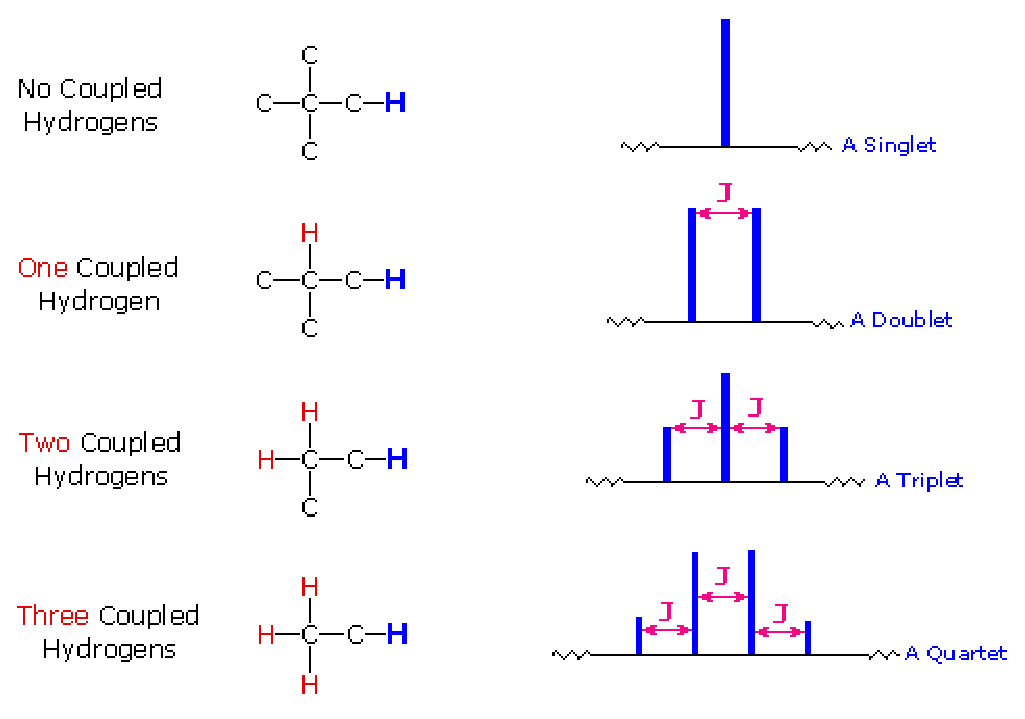
\includegraphics[width=0.7\textwidth]{espectro_coupling}
   \caption{Representación esquemática de los espectros referentes al H en azul. Cada uno de los H en rojo representa un núcleo emparejado con el H azul (con la misma J).}
 \label{fig:espectro_coupling}
 \end{figg}
\end{figure}







\begin{figure}[htb]
 \begin{figg}
   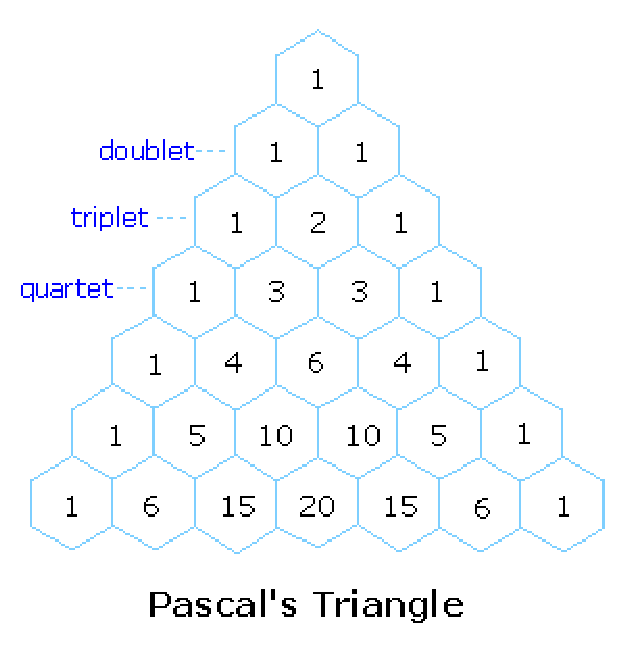
\includegraphics[width=0.7\textwidth]{espectro_pascal}
   \caption{El triángulo de Pascal es un gráfico que se utiliza, en RMN, para predecir el ratio de altura entre los picos de spines separados en el espectro. Puede observarse que cada hexágono representa la suma de los dos hexágonos contiguos superiores.}
 \label{fig:espectro_pascal}
 \end{figg}
\end{figure}

 




\begin{figure}[htb]
 \begin{figg}
   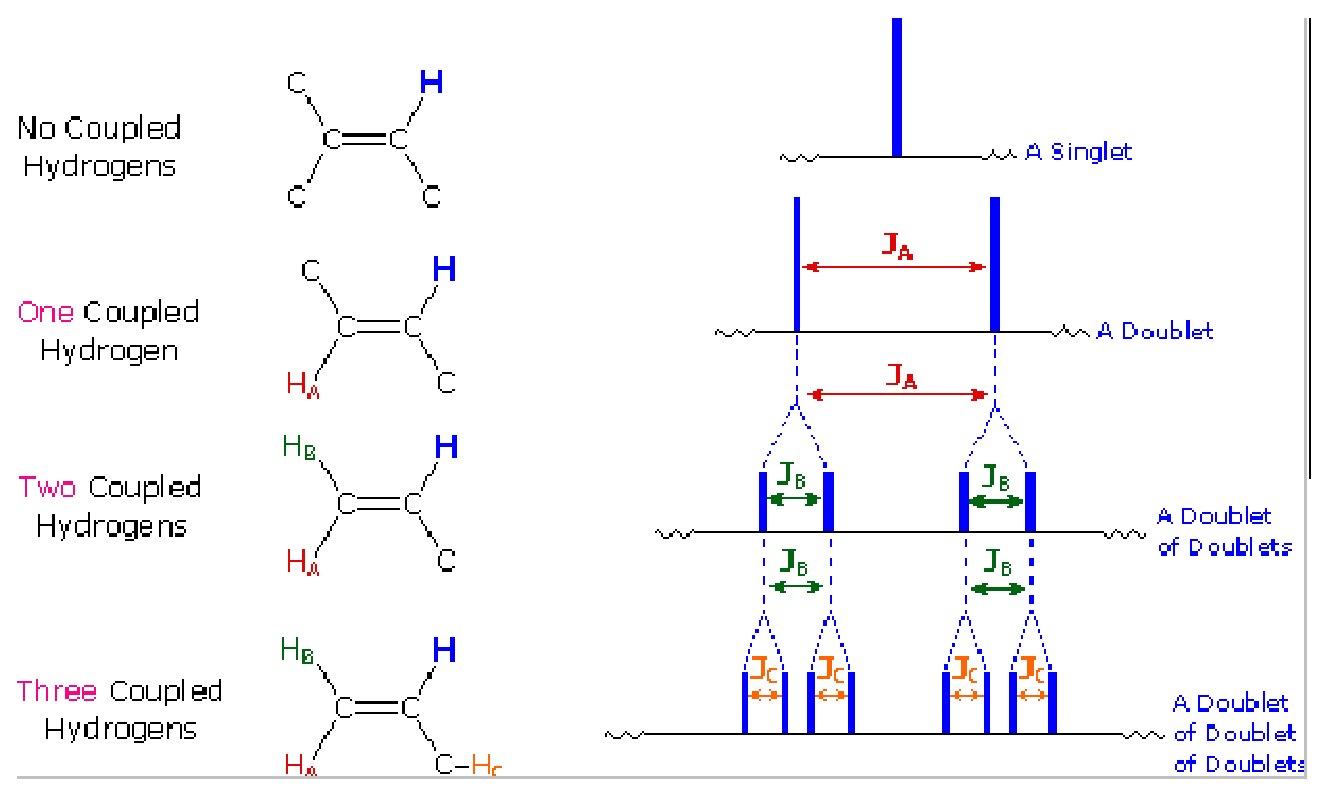
\includegraphics[width=0.7\textwidth]{espectro_couplingComplex}
   \caption{Las diferentes interacciones entre los núcleos lleva a configuraciones más complejas, como se muestra en la imagen. Cada H de un color representa una constante J distintinta (del mismo color al H).}
 \label{fig:espectro_couplingComplex}
 \end{figg}
\end{figure}





A pesar de que esta técnica solo detecte protones de H, podemos aprovechar las características del espectro anteriormente mencionadas para poder determinar los componentes presentes en la muestra, ya que podemos detectar la cantidad de protones de H y diferenciar los que no son isocrónicos y saber del emparejamiento de estos. Además podemos comparar el espectro resultante con otros espectros ya realizados, pudiendo consultar una base de datos de espectros preexistente.


\section{Espectroscopía por RMN in vivo}
Al igual que las técnicas de iRMN para la espectroscopía por RMN requiere de:

\begin{itemize}
  \item Un intenso campo magnético homogéneo
  \item Un transmisor de Radio Frecuencia capaz de producir pulsos cortos
  \item Un receptor sensible para amplificar al señal de RMN
  \item Un digitalizador de la señal 
  \item Un programador de pulsos
  \item Una computadora para el control y análisis de los datos
  \item Un ``contenedor'' que permita la excitación de la muestra a través de las bobinas
\end{itemize}


Sin embargo el contenedor de la muestra no tiene por qué ser un contenedor físico. Gracias a las técnicas de codificación espacial de iRMN podemos establecer un contenedor virtual que delimite un área de interés y solo recibiremos señal de dicha muestra contenida. Gracias a este proceso podemos realizar espectroscopía por RMN in vivo, ya que no necesitamos extraer físicamente la muestra del paciente (como en una biopsia). El contenedor virtual no es más que un voxel, el cual podemos determinar su tamaño y localización gracias a gradientes en la magnetización. A diferencia de iRMN, donde se excita selectivamente una rebanada y con gradientes de magnetización se obtiene una señal que luego se codifica espacialmente (dentro de esa rebanada), en la espectroscopía por RMN  se excita selectivamente tres planos ortogonales y es donde estos tres se superponen que queda determinado el voxel o volumen de interés (y por tanto será el único lugar de donde tendremos señal). Este método se llama SVS (single Voxel Spectroscopy)

\begin{figure}[htb]
 \begin{figg}
   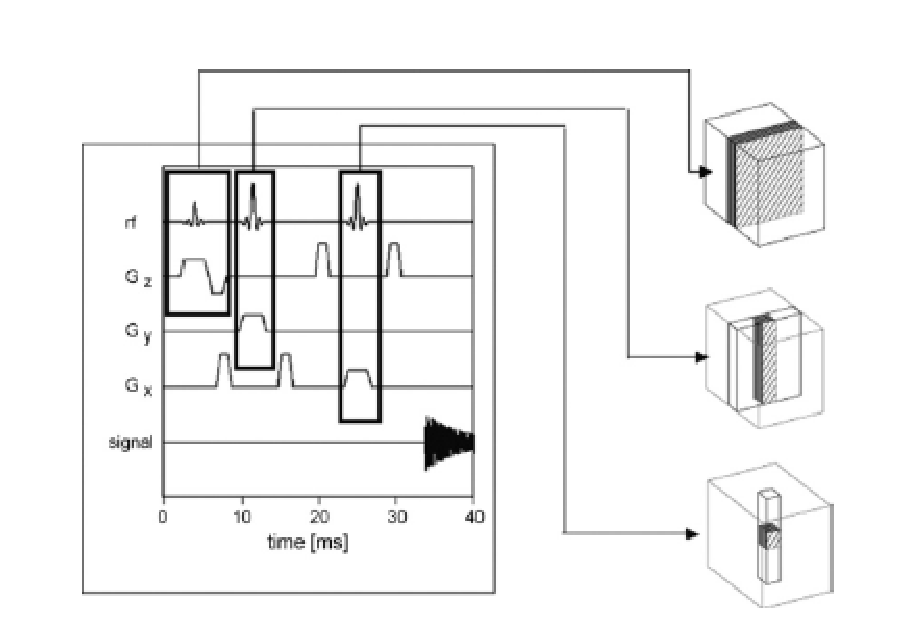
\includegraphics[width=0.7\textwidth]{espectro_singleVoxel}
   \caption{Esquema representativo de la secuencia para la obtención de un voxel o volumen de interés. Observese que el voxel resultante es producto de la superposición de los 3 planos ortogonales. Este voxel será el único volumen que reciba todos los requisitos para emitir señal.}
 \label{fig:espectro_singleVoxel}
 \end{figg}
\end{figure}





En espectroscopía por RMN se utilizan principalmente dos secuencias PRESS (pointed-resolved spectroscopy) y STEAM (stimulated echo acquisition mode).


\subsection{PRESS}
La secuencia más utilizada es PRESS. En esta, el espectro se obtiene con un pulso de 90º seguido de otros dos de 180\degrees. Cada uno de ellos es aplicado al mismo tiempo con diferentes gradientes magnéticos. Entonces, la señal emitida por el voxel es un spin eco. El primer pulso de 180\degrees se aplica después de un tiempo $1/2TE$ después del primer pulso de 90\degrees, i el segundo pulso de 180\degrees se aplica después de un tiempo $1/2TE + TE$. La señal se produce después del tiempo $2TE$. Para restringir la adquisición a un solo voxel, se requieren gradientes destructores. Los gradientes destructores desfasan los núcleos fuera del voxel de interés y reducen la señal.



\begin{figure}[htb]
 \begin{figg}
   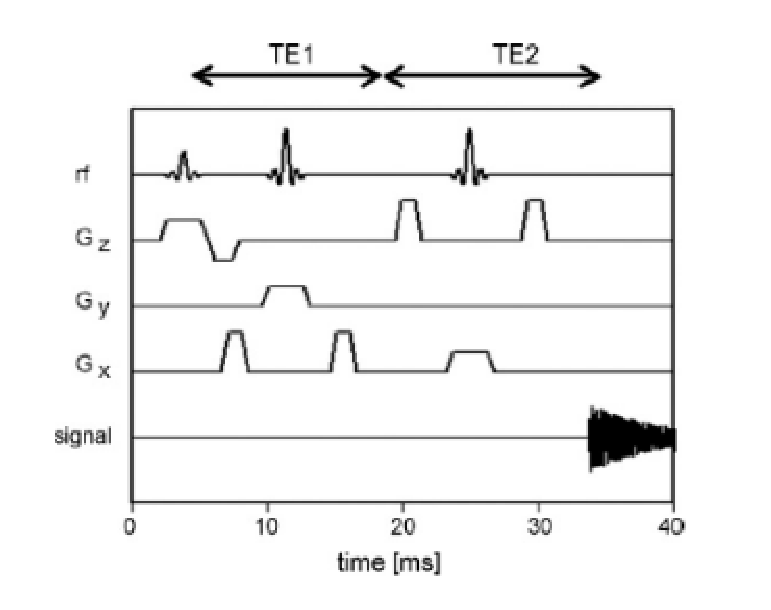
\includegraphics[width=0.7\textwidth]{espectro_press}
   \caption{Secuencia PRESS.}
 \label{fig:espectro_press}
 \end{figg}
\end{figure}






\subsection{STEAM}
Dado que la secuencia STEAM solo usa pulsos de 90\degrees, tiene un 50\% menos de ratio señal-ruido (SNR, de signal-noise ratio) que PRESS.  Los pulsos de 180\degrees  resultan en un voxel menos óptimo y conllevan un SNR más alto. Sin embargo, dado que la longitud de los pulsos de 180º son más largos, PRESS no se puede hacer con TE muy cortos. Otro inconveniente de PRESS es que tiene un mayor artefacto de desplazamiento por corrimiento químico.

\begin{figure}[htb]
 \begin{figg}
   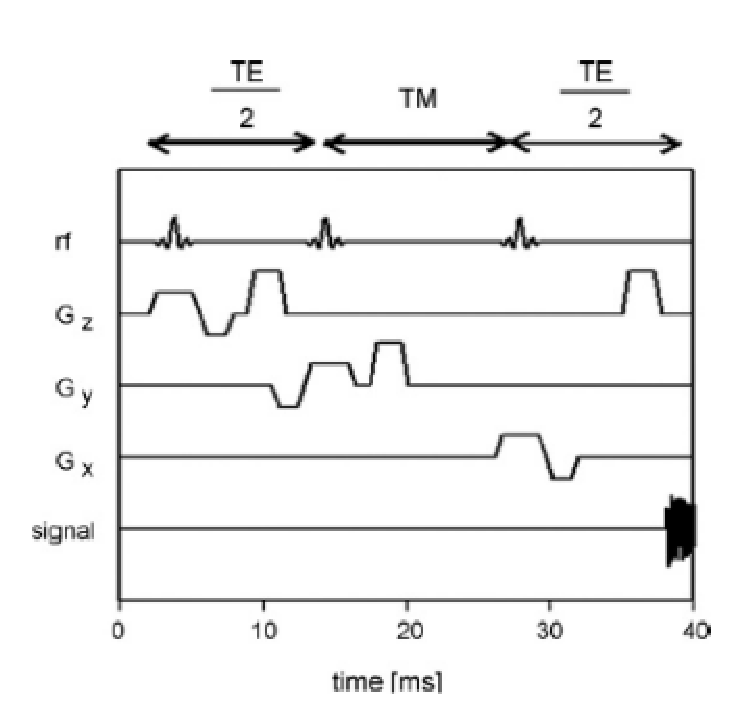
\includegraphics[width=0.7\textwidth]{espectro_steam}
   \caption{Secuencia STEAM.}
 \label{fig:espectro_steam}
 \end{figg}
\end{figure}


Si nos interesa un estudio de la distribución espacial (y no de un solo voxel) es posible realizar una espectroscopía multivoxel (MVS) e incluso de puede obtener unas imágenes de espectroscopía de resonancia magnética (MRSI). A diferencia de las imágenes iRMN, el resultado final es una matriz (2D o 3D) con los espectros de cada uno de los voxeles. Para ello solo se requiere un gradiente codificador de fase después del pulso RF en cada una de las dimensiones que se quiera codificar.

Las técnicas SVS resultan en espectros de alta calidad, en un tiempo de escáner corto, y buena homogeneidad de campo. Es decir SVS se utiliza para obtener mediciones precisas de metabolitos. Por otro lado las técnicas MRSI presentan la ventaja de además tener información relativa a la distribución espacial, pero la cuantificación de metabolitos no es tan precisa debido al sangrado de voxeles (el espectro dado por un voxel puede presentar contribución de otras regiones espaciales). Por eso MRSI se suele utilizar para determinar heterogeneidad espacial.

% SVS
% MRSI
% TE corto
% TE largo
% 1 voxel
% Multi-voxel
% Región limitada
% Adquisición múltiple de datos
% Área fija
% Cuadrícula movible tras adquisición
% Más precisa
% Sangrado del voxel
% Mediciones cuantitativas
% Distribución espacial


\subsection{TE para MRS}
Las MRS se pueden obtener con diferentes TE, dando diferentes espectros.
Con TE cortos (20-40ms) tienen mayor SNR y menos pérdida de señal debido al peso de T2 y T1 (en comparación con TE largos). Así pues los espectros con TE cortos presentan más picos de metabolitos, que no se detectan con espectros de TE largos. Sin embargo dado el mayor número de picos, estos puede presentar solapamiento (importante tener en cuenta a la hora de cuantificar).
Con TE largos (135-288 ms) hay peor SNR, sin embargo tienen espectros más simples debido a la supresión de señal. 


\begin{figure}[htb]
 \begin{figg}
   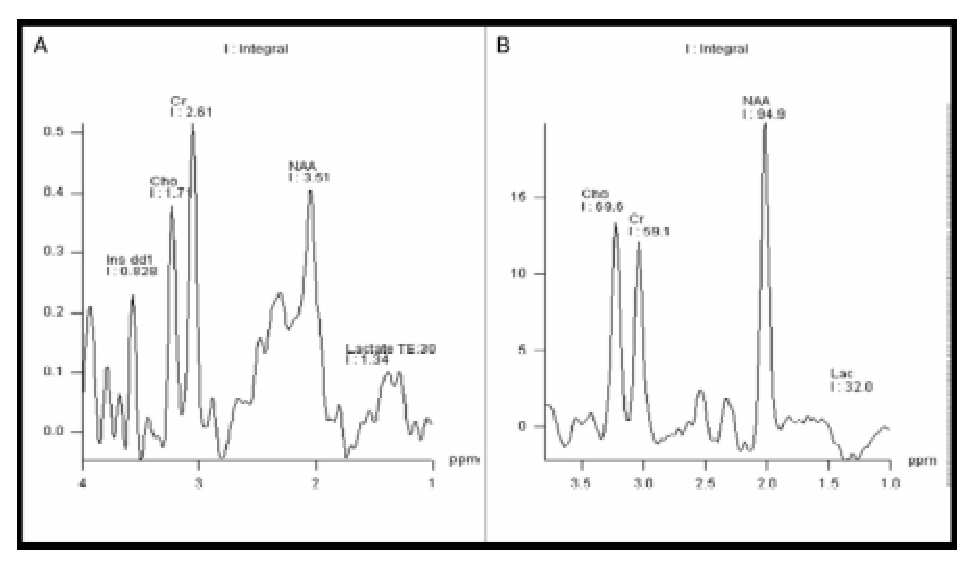
\includegraphics[width=0.7\textwidth]{espectro_TEs}
   \caption{Comparación entre dos espectros de la misma muestra con diferentes TE. A) Espectro con TE=30 ms. B) Espectro tomado con TE=135 ms.}
 \label{fig:espectro_TEs}
 \end{figg}
\end{figure}






En cerebro el agua es muy abundante, siendo su señal en el espectro de MRS mucho más alta que los otros metabolitos. Para evitar la superposición del pico del agua con otros picos de otros metabolitos se requiere de técnicas de supresión de la señal de agua.

\begin{figure}[htb]
 \begin{figg}
   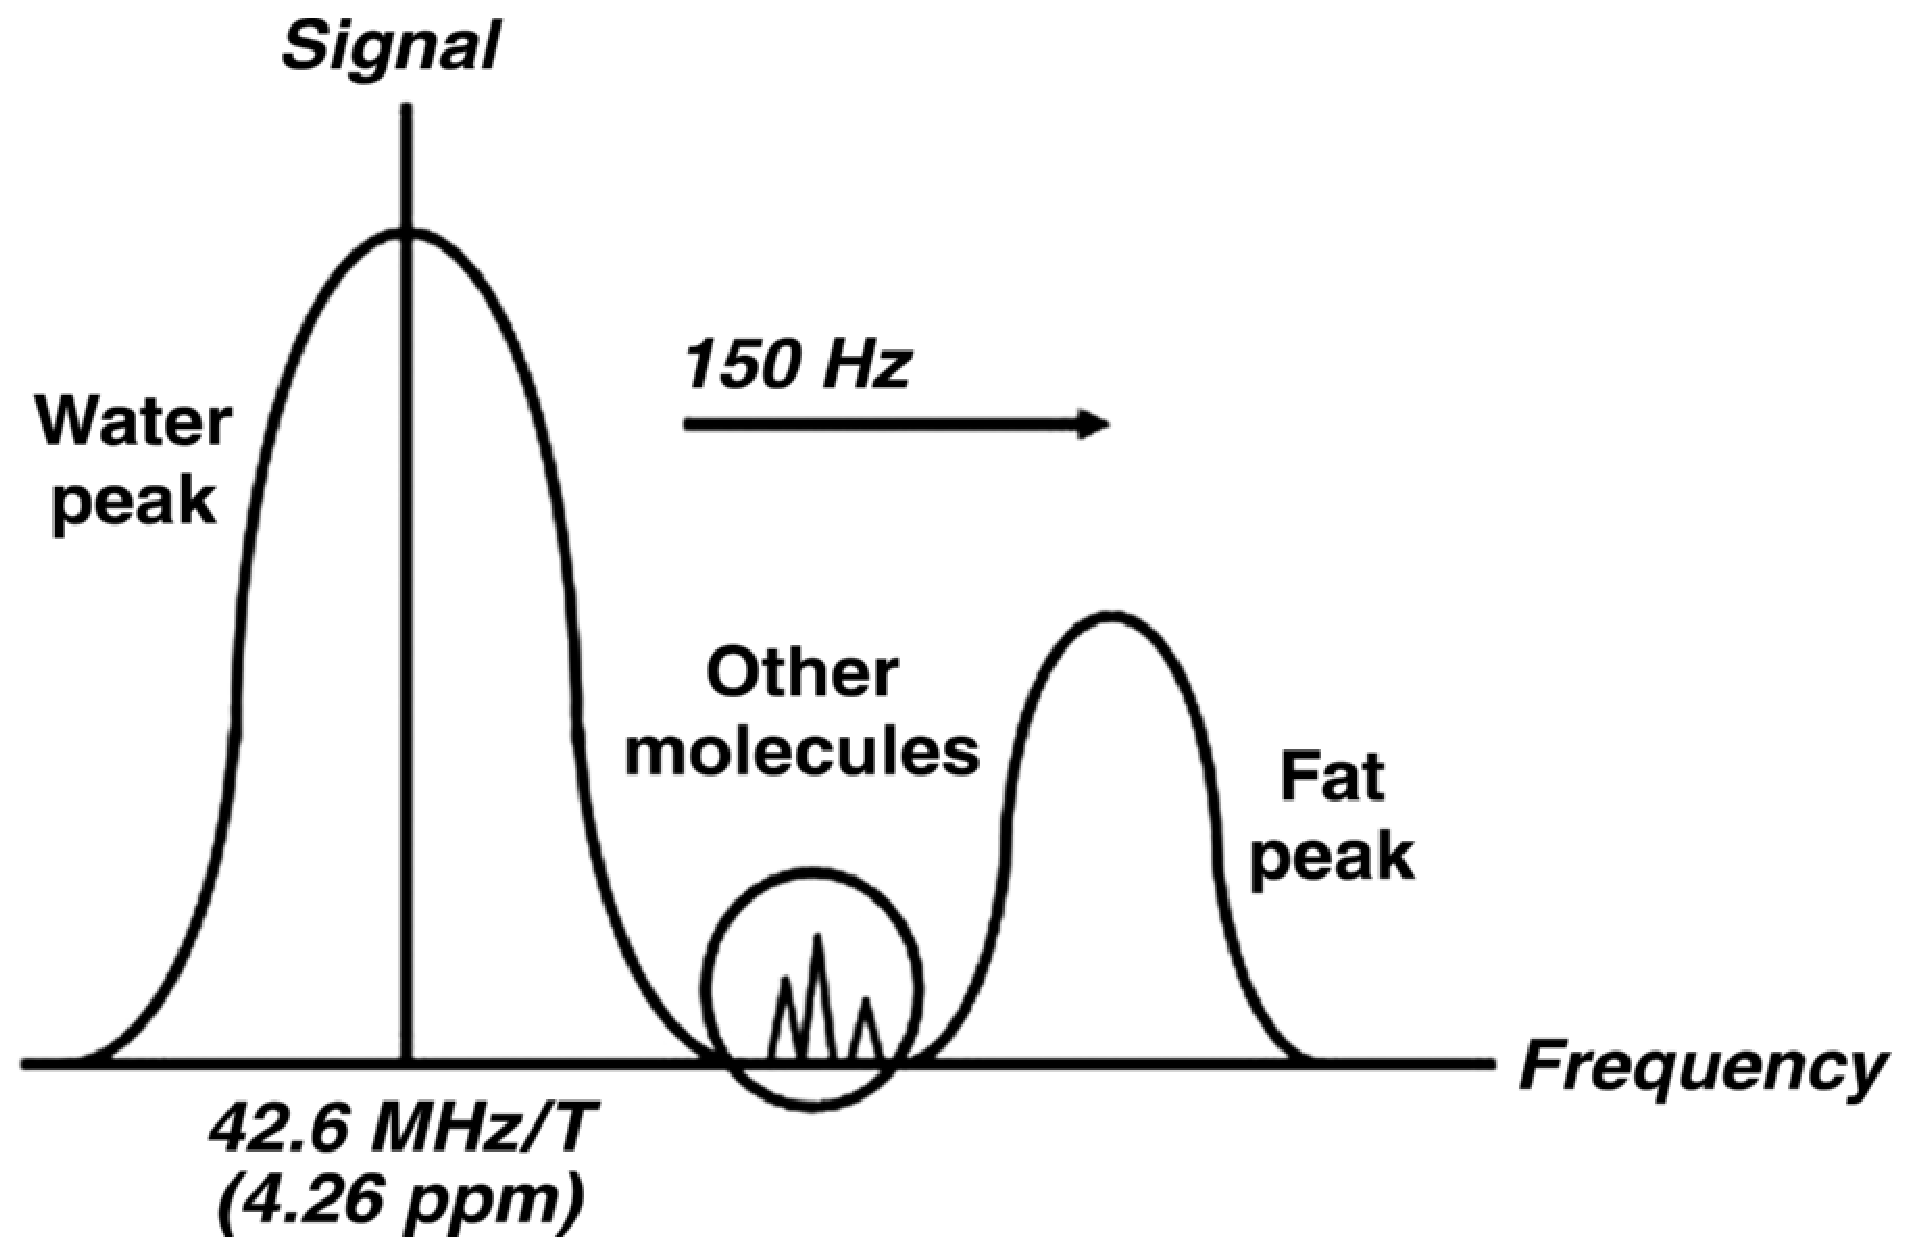
\includegraphics[width=0.7\textwidth]{espectro_aguaLipido}
   \caption{Como se observa en el gráfico, la señal obtenida de agua y lípidos son mucho mayores que las moléculas de interés en espectroscopía. Es por eso que se requiere de mecanismos para evitar que su señal enmascare o influya de algún modo en el espectro.}
 \label{fig:espectro_aguaLipido}
 \end{figg}
\end{figure}




La secuencia más común para ello es CHESS (chemical shift selective water suppression), en la cual se pre-satura la señal del agua usando frecuencias selectivas de pulsos de 90º antes de la secuencia de pulsos de localización. Otra secuencia es VAPOR (VAriable Pulse power and Optimized Relaxation Delays) y WET (Water suppression Enhanced Through T1 effects)

\begin{figure}[htb]
 \begin{figg}
   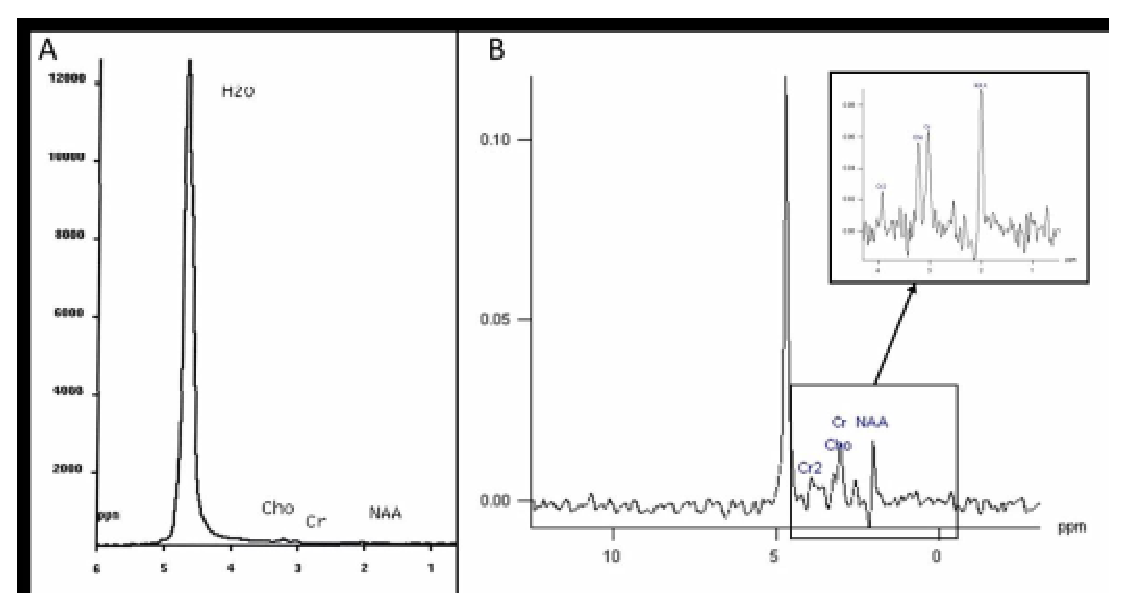
\includegraphics[width=0.7\textwidth]{espectro_CHESS}
   \caption{Comparación entre espectros con y sin suprimir la señal del agua. Antes de la secuencia CHESS (A) y después de la secuencia CHESS (B).}
 \label{fig:espectro_CHESS}
 \end{figg}
\end{figure}




\section{Artefactos en espectroscopía por RMN}
La espectroscopía por RMN también está sujeta a la aparición de artefactos. Des de la mala supresión de la señal de agua o lípidos, inhomogeneidad del campo magnético, corrientes de Eddy a desplazamiento por corrimiento químico, son algunos de los factores que introducen artefactos en espectro.
Lo más importante es la homogeneidad del campo magnético, pues una baja homogeneidad reduce el SNR y aumenta la anchura de los picos. Algunos lugares son más susceptibles a este fenómeno, cerca del hueso o de interficie tejido-aire. Se recomienda evitar estos lugares al determinar nuestro Volumen de interés.
Los corrientes de Eddy que se causan por el encendido de los gradientes, provocan también artefactos. Un corriente de transito resulta en la distorsión de la forma de los picos, haciendo difícil la cuantificación del espectro.
El desplazamiento por corrimiento químico puede provocar artefactos. La localización del voxel está basada en la frecuencia de precesión de los protones. Dado que estas frecuencias son diferentes para cada metabolito, la posición exacta de dichos metabolitos será ligeramente diferente. Para resolver este problema, se requiere de gradientes de campo fuertes para la selección de rebanada.




\section{Metabolitos en el cerebro}
La espectroscopía por RMN permite la detección de metabolitos en el cerebro. Cambios en estos metabolitos delatan anormalidades estructurales. Para saber de estos cambios se requiere conocer los espectros del cerebro en estado normal y sus diferentes variantes dependiendo de técnicas, edad del sujeto, regiones cerebrales, etc.
A continuación trataremos algunos metabolitos de interés analítico en el cerebro, y la Tabla \ref{tab_espectro_metabolitos} muestra un resumen de los hallazgos más comunes en espectroscopía en presencia de anormalidades tisulares específicas.

\subsection{N-acetilaspartato (NAA)}
El pico de NAA es el más alto del espectro del cerebro normal. Este pico está alrededor de  2,02 ppm. Se sintetiza en la mitocondria de las neuronas y es transportado al citoplasma a lo largo del axón. Es un metabolito exclusivo del sistema nervioso central (SNC), tanto en sustancia blanca como gris. Es un marcador de densidad y viabilidad neuronal y axonal. Puede encontrarse en oligodendrocitos inmaduros y células progenitoras de astrocitos.
La ausencia o reducción de la concentración de NAA es señal de pérdida o degradación neuronal. Por otro lado, su incremento es específico de la enfermedad de Canavan.

\subsection{Creatina (Cr)}
El pico de Cr se asigna a 3,02 ppm. Este pico representa una combinación de moléculas que contienen  creatina y fosfocreatina. Es un marcador metabólico intracelular y del sistema energético. La concentración de Cr es relativamente constante y muy estable. Se utiliza como referencia interna para calcular ratios con otros metabolitos.
En tumores cerebrales, hay reducción de la señal de Cr. Por otro lado la gliosis puede producir un incremento mínimo, dado el incremento de la densidad de células gliales (proliferación de la glia). Enfermedades sistémicas pueden afectar también la concentración de CR en el cerebro.

\subsection{Colina (Cho)}
Se asigna al pico de 3,22 ppm y representa la suma de Cho y compuestos que contengan Cho. Es un marcador de recambio de la membrana celular, reflejando proliferación celular. En tumores, los niveles de Cho correlacionan con el grado de malignidad. El aumento de Cho pude aparecer también en infarto o inflamación.
Lactato (Lac)
El pico del Lac no parece en un espectro del cerebro “normal”, o es casi inapreciable. EL pico del Lac es un doblete en 1,33 ppm, el cual proyecta por encima de la línea base cuando se adquiere con TE cortos/largos, pero se invierte con TE de 135-144 ms. Lac se produce por glicolisis anaeróbica, por tanto su presencia en cerebro indica hipoxia, isquemia, epilepsia y desordenes metabólicos. También hay aumento por acumulación de macrófagos (inflamación). Este también se acumula en tejidos con bajo recambio de fluido, como cistos.

\subsection{Lipidos (Lip)}
Los Lipidos son componentes de membrana, estos no pueden ser visualizados con TE largos, debido a su corto tiempo de relajación. Hay dos picos de lípidos: a 1,3 ppm se encuentra los que contienen grupos metilenos, y a 0,9ppm los que contienen grupos metil. Estos picos están ausentes en el cerebro normal. Los picos de lípidos pueden observarse cuando se rompe la membrana celular o por necrosis, como ocurre en metástasis y tumores malignos.

\subsection{Mioinositol (Myo)}
Myo es un azúcar simple asignado al pico 3,56 ppm. Se considera un marcador glial dado que es principalmente sintetizado en células gliales (prácticamente solo astrocitos). Es también el osmolito más importante en astrocitos. Myo puede representar el producto de la degradación de la mielina. Altos niveles de Myo se presentan cuando ocurre una proliferación de células gliales o aumento del tamaño de estas (inflamación). Los niveles de Myo se presentan elevado en gliosis, astrocitosis y la enfermedad de Alzheimer.

\subsection{Alanina (Ala)}
Ala es un aminoácido que presenta un doblete centrado en 1,48 ppm. Este pico se encuentre por encima de la línea base en espectros adquiridos con TE corto/largo, y se invierte por debajo cuando se adquiere con TE de 135-144 ms. Su pico puede verse enmascarado por Lac (a 1,33 ppm). LA función de Ala es incierta pero juega un rol en el ciclo del ácido cítrico. Un aumento en la concentración de Ala puede ocurrir por algún defecto en el metabolismo oxidativo. En tumores este aumento es específico de meningiomas.
Glutmato-Glutamina (Glx)
Glx es un pico complejo de Glutamato (Glu), Glutamina (Gln) y ácido gamma-aminobutírico asignado al pico de 2,05 a 2,50 ppm. Estos metabolitos son muy difíciles de separar a 1,5T. Glu es un neurotransmisor excitatorio muy importante y también juega un papel en el ciclo redox. Concentraciones elevadas de Gln se encuentran en algunas pocas enfermedades como en encefalopatía hepática.
El principal uso de la espectroscopía por RMN del cerebro es el de diagnóstico. Gracias a la espectroscopía por RMN se pueden observar cambios en los metabolitos previamente nombrados, con la enorme ventaja de no necesitar abrir el cráneo.



\begin{table}[htbp]
\centering
\caption{Tabla que muestra diagnosis de tumores en base a cambios en el espectrode RMN. \textuparrow  Pico aumentado; \textdownarrow  Pico disminuido; N Pico normal. 1: NAA ausente en el centro del tumor. 2: La presencia de Lac depende del grado del tumor. 
3: Lac y Glu se encuentran aumentados solo en estados iniciales de la enfermedad.}
\label{tab_espectro_metabolitos}
\begin{tabular}{@{}lcccccccccc@{}}
\toprule
                     & Cho & NAA & Lac & Lip & Myo & Glu & Suc & Acet & Ala & Aa \\ \midrule
Tumor de bajo grado  & \textuparrow   & \textdownarrow   &     &     & \textuparrow   &     &     &      &     &    \\
Tumor de alto grado  & \textuparrow   & \textdownarrow   & \textuparrow   & \textuparrow   &     &     &     &      &     &    \\
Metastasis           & \textuparrow   & \textuparrow$^1$  & \textuparrow   & \textuparrow   &     &     &     &      &     &    \\
Oligodendroglioma    & \textuparrow   & \textdownarrow   & \textuparrow$^2$  &     &     &     &     &      &     &    \\
Meningioma           & \textuparrow   & \textuparrow   &     &     &     &     &     &      & \textuparrow   &    \\
Gliomatosis cerebral & \textuparrow   & \textdownarrow   &     &     &     &     &     &      &     &    \\
Linfoma              & \textuparrow   & \textuparrow$^1$  &     & \textuparrow   &     &     &     &      &     &    \\
Radionecrosis        & \textdownarrow   & \textdownarrow   & \textuparrow   & \textuparrow   &     &     &     &      &     &    \\
Abcesos              & N   & \textdownarrow   & \textuparrow   & \textuparrow   &     &     & \textuparrow   & \textuparrow    & \textuparrow   & \textuparrow  \\
Desmelinización      & \textuparrow   & \textdownarrow   & \textuparrow$^3$  & \textuparrow   & \textuparrow   & \textuparrow$^3$  &     &      &     &    \\ \bottomrule
\end{tabular}
\end{table}




% Lecturas recomendadas
% The basics of MRI, Joseph P. Hornak (1996-2014).
% 1H MR Spectroscopy of the Brain: Absolute Quantification of Metabolites, Jacobus F. A. et al., Radiology (2006).
% Brain Proton Magnetic Resonance Spectroscopy, Débora Bertholdo, University of North Carolina at Chapel Hill. *(http://www.ajnr.org/site/fellows/files/MRS-chapter-Castillo.pdf)
% MRI From Picture to Proton, Donald W. McRobbie et al., Cambridge University Press 2ª Ed. (2006).
% 
% Páginas web recomendadas
%  http://orgchem.colorado.edu/Spectroscopy/
% http://www-keeler.ch.cam.ac.uk/lectures/Irvine/
% https://www2.chemistry.msu.edu/faculty/reusch/virttxtjml/Spectrpy/spectro.htm